



\section{Introduction and related work}
Language Modeling (LM) is one of the numerous essential parts of modern Natural Language Processing (NLP). Language modeling is the task of assigning a probability to sequences in a language. Apart from assigning a probability to each sequence of words, the language model assigns a probability for a given word or a sequence of words to follow a sequence of words \cite{Goldberg2017}. Our specified task is to train such model, and generate best text possible with lowest perplexity (LM models quality measure). We are required to use novel techniques beyond basic vanilla RNN methods. 

To narrow scope of related works to our solution, we will focus only on breakthrough papers based mainly around attention blocks. Transformers have provided state-of-the art results within this field for past few years. This architecture has been firstly proposed in  \cite{DBLP:attention}, and was since basis of modern LM. Attention mechanism is crucial part of these models as the most important component for learning long range dependencies in text delivering better results than statistical methods, while avoiding causal training constraint of Recurrent Neural Networks (RNN). GPT \cite{radford2018improving:gpt} has been one of the first LM which demonstrated usage of this architecture. GPT was was at the time one of the best LM models to date. Achieving superior results thanks to having massive amount of parameters and largest training data set at the time. BERT \cite{DBLP:bert} has later introduced usage of bidirectional attention while also introducing training processes different to GPT. BERT analyzes sequence from both direction to get both left and right context, which achieves state-of-the-art results for range of tasks. The limitations of these networks have lead to development of different approaches to attention mechanism itself, one of which is called Performer \cite{DBLP:performer}. Performer improves to linear time and space complexity from quadratic complexity of classical attention.

\section{Transformer architecture}
Transformer architecture proposes two interlinked neural networks. The roles between two networks are split into encoder and decoder. The role of the encoder network is to create a embedding of the input sequence. This embedding among with beginning of target sequence is later used as input for decoder network. 

Both of these networks are similar in nature, since both use multi-head attention. The main difference between the two is within usage of masked attention. Masking provides a way for attention mechanism to only focus on the words which appeared before a certain word, making it look only to the past. This mechanism is used for decoder network since it cannot know the relations to words which will be generated. The encoder on the other hand can look at the sentence as a whole, deeming masking not necessary.

Depending on the specific case, language models use one or another attention mechanism. Our specific implementation uses a decoder network similar to GPT model used in \cite{radford2018improving:gpt}. Except of the obvious architectural difference the decoder based language models differ in the way they are being trained. Our model is trained on the input sequence with a desired output offset by one symbol into the future. This way the model trains to predict next word given words before it. Masked attention or self-attention makes is in this case beneficiary since future words will be predicted and thus are not known. The overall architecture of used decoder layer can be seen on Figure \ref{fig:architecture}.

\begin{figure}[h]
    \centering
    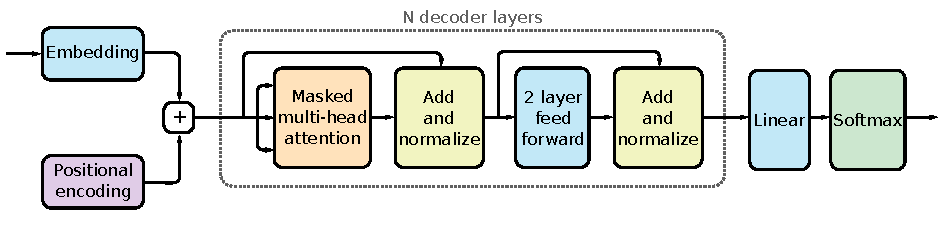
\includegraphics{obrazky/language_model_architecture.pdf}
    \caption{Language model architecture}
    \label{fig:architecture}
\end{figure}

\section{Multi-head attention mechanism}
\label{sec:mha}

A multi-head attention, is a extension of simple attention where different parallel instances of attention layer focus on different dimension of input. The input is in this case split into predefined number of instances, which equals to the number of heads. The dimension of single instance can be then determined as $d_{head} = {\frac{d_{model}}{n_{head}}}$, where $d_{model}$ is number of dimensions provided by embedding layer and $n_{head}$ is number of heads in multi-head attention mechanism. To make multi-head processing effective, one more dimension is added input. Output is later flattened.

The input processing is firstly preceded by three parallel linear layers. Reason for these layer is to create three different input sequences described as $Q,K,V \in \mathbb{R}^{s_{len} \times d_{head}}$, where $Q$ are considered to be queries, $K$ keys and $V$ values. The method first computes how well certain key reflects the query, creating a matrix with size of $s_{len} \times s_{len}$ in process. The matrix is then passed through scaling and masking layers. Results are then passed through a soft-max function thus creating weight matrix $A$. Values matrix multiplied by $A$ matrix give results in the form of best matched values according to given queries and keys. Diagram of single head can be seen on Figure \ref{fig:multi-head}.

\begin{figure}[h]
    \centering
    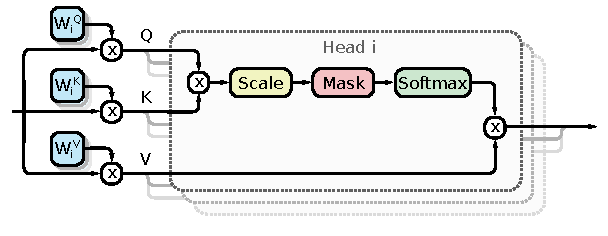
\includegraphics[height=4cm, width=10.3cm]{obrazky/multi_head_attention.pdf}
    \caption{Multi-head attention}
    \label{fig:multi-head}
\end{figure}

As can be seen the multi-head attention layer has by itself three trainable weight matrices $W^Q_i, W^K_i, W^V_i \in \mathbb{R}^{d_{model} \times d_{head} }$. Our implementation combines these matrices for all heads into three matrices for entire multi-head attention mechanism so that $W^Q, W^K, W^V \in \mathbb{R}^{d_{model} \times d_{model} }$. The split for different heads is done with another added dimension and view of returned data. However in later equations only original way is used. Attention for single head is formally described in the Performer publication as follows:
\begin{equation}
    Att(Q,K,V)=D^{-1}AV,\ 
    A = exp(QK^T/\sqrt{d_{head}}),\ 
    D=diag(A1_{s_{len}}),
\end{equation}
where $D$ represents sum of rows within a $A$ matrix in a diagonal matrix form, and thus $D^{-1}$ represents normalization for a softmax function. Our reference implementation uses a soft-max directly and does not compute n this way. Matrix $D^{-1}A \in \mathbb{R}^{s_{len} \times s_{len}}$, contains weights described in previous section. 

As can be seen the complexity of this computation is highly depended on the $s_{len}$, where the time complexity to compute matrix $AV$ can be described as $O(s_{len}^2 d_{head} + s_{len}^2 d_{head})$, thus having quadratic time but also space complexity.
\section{Linear time complexity using a FAVOR+}
\label{sec:performer}
The quadratic time complexity is where authors of \cite{DBLP:performer} propose a effective and accurate linearization of attention mechanism. The main idea of this approach is to utilize fact that if soft-max function used to calculate weights could be approximated using matrix multiplication the attention equation could be rewritten as:
\begin{equation}
    Att(Q,K,V) = \Hat{D}^{-1} (Q'((K')^T V)),\ 
    \Hat{D} = diag(Q'((K')^T 1_{s_{len}}))
\end{equation}
The time complexity is thus reduced since multiplication of matrices $Q'((K')^T V)$ has time complexity of $O(s_{len} d_{head}^2 + s_{len} d_{head}^2)$, thus making it linear, in relation to $s_{len}$ but quadratic to $d_{head}$. This promises better performance among longer input sequences, which may not be possible due to computational limitation with classical attention mechanism.

This publication suggests an innovative method of creating projections $Q'$ and $K'$, so accuracy of attention mechanism stays. Previous methods have tried similar approaches but often failed to deliver needed accuracy in specific values. These inaccuracies lead to performance incomparable to classical attention mechanism. Estimation of attention is done via positive orthogonal random features and thus the name \textit{Fast Attention Via positive Orthogonal Random features (FAVOR+)}. 

The features are a result of projection of original values of $Q$ and $K$ into space where multiplication results in soft-max estimation. The general approach can be described as:
\begin{equation}
    \phi(x) = \frac{h(x)}{\sqrt{m}} (f_1(\omega_1^T x), \dots ,f_1(\omega_m^T x), \dots ,f_n(\omega_1^T x),\dots,f_n(\omega_m^T x) )
\end{equation}
Where projection $\phi(x)$ of vector $x$ of given dimension $d$, is describes as multiple projection using function $f$ of inner dot product of $x$ with different random vectors $\omega$. The number of vectors $\omega$ and number of functions $f$ is by general definition arbitrary. The specific instance of such projection is proposed. Authors propose usage of vectors randomly drawn from normal distribution $\omega_1,\dots,\omega_m \sim \mathcal{N}(0,I_d)$, where $I_d$ is identity matrix of dimension $d$. In addition vectors $\omega_1,\dots,\omega_m$ are orthogonalized using Gam-Schmidt method. Our implementation uses $qr$ method available in \textit{PyTorch} framework. The number of vectors is arbitrary an can be even larger than $d$, but organization need to be done on multiple slices of size $d$ and later concatenated into single matrix, for effective projection computation.

Authors propose usage of a one function $f$ which is simply described as $f(x) = exp(x)$. The $h(x)$ is proposed as:
\begin{equation}
    h(x) = \frac{1}{\sqrt{2}} exp(-\frac{||x||^2}{2})
\end{equation}

Our implementation wraps whole projection into single method which on call will produce projected features for given batch of input sequences. It uses a soft-max kernel described in previous section with function and orthogonal features created according to authors recommendation. Additionally authors recommend so called \textit{redrawing} of orthogonal random features which is done every $4000$ iterations.

Multiplication of projected features can produce directly a bi-directional attention mechanism. Self-attention used for our language model needs a different approach. The method of masking used in classical multi-head attention cannot be used directly. This is mainly because this approach is not producing the $A$ matrix an thus it cannot be masked. Authors provide a solution to this problem which introduces the use of prefix sums. Two method are described in implementation provided by authors and they describing the process of creating masked attention. First one is used to create so called casual numerator, or the $Q'(K')^T V$ matrix.

\begin{algorithm}[H]
\SetAlgoLined
\KwResult{Return numerator for self-attention }
 $result \leftarrow EmptyList$\;
 $S \leftarrow ZerosMatrix(d_{head}, d_{head})$\;
 \For{$i$ \textbf{in} $Range(0,s_{len})$}{
  $S \leftarrow sums + (K')[i] ((V')[i])^T$\;
  $result.append(S\ (Q')[i])$\;
 }
 \Return{$result$}
 \caption{CasualNumerator}
 \label{alg:cn}
\end{algorithm}
The Algorithm \ref{alg:cn} uses $X[i]$ to index $i$-th item in the sequence. The dimension of items within $V$ and $Q$ are considered to be equal. The other method creates normalizations for values created in Algorithm \ref{alg:cn}, hence the name casual denominator. 

\begin{algorithm}[H]
\SetAlgoLined
\KwResult{Return denominator for self-attention }
 $result \leftarrow EmptyList$\;
 $S \leftarrow ZerosMatrixLike((K')[0])$\;
 \For{$i$ \textbf{in} $Range(0,s_{len})$}{
  $S \leftarrow sums + (K')[i] $\;
  $result.append(InnerDotProduct((Q')[i], S))$\;
 }
 \Return{$result$}
 \caption{CasualDenominator}
 \label{alg:cd}
\end{algorithm}
A reference implementation in \textit{Python}, which is given by author and is described above differs in some cases from original \textit{FAVOR+} defined in the paper. The differences are however formal and are mainly in the usage of $C$ matrix instead of $V$ which is equivalent to $C = [V\ 1_{s_{len}}]$. This makes it possible do discard Algorithm \ref{alg:cd}, because added 1 will make equivalent role to $InnerDotProduct$. Using this approach it is however necessary to later split results into numerator and denominator parts. As for original algorithm the resulting attention can be simply computed as:
\begin{equation}
    Att(Q,K,V) = diag(CasualDenominator)^{-1} CasualNumerator
\end{equation}

\section{Implementation}

Our implementation contains both method for providing attention the classical multi-head attention presented in Section \ref{sec:mha} and linear attention mechanism described in Section \ref{sec:performer}. The implementation environment is \textit{Python} wih a version \textit{3.8+}. We have chosen \textit{PyTorch} framework accompanied by \textit{PyTorch Lightning} in order to provide efficient training and inference environment. The whole implementation can be seen in our \textit{GitHub repository}\footnote{\url{https://github.com/karabellyj/KNN2021-LM}}. 

The implementation is bases out of multiple sources which were used for reference. The transformer network architecture used for purposes of language modeling is loosely based out of implementation provided directly in \textit{PyTorch} with module \texttt{TransformerDecoder}. The source code of which can be seen in \textit{PyTorch GitHub repository}\footnote{\url{https://github.com/pytorch/pytorch/blob/master/torch/nn/modules/transformer.py}}. The network has been re-implemented from ground up to suit specific needs of language model. The original decoder network is suitable for sequence to sequence modeling and thus requires input of values. In order to make it so values are not needed and are taken from inputs of the decoder layer, the provided architecture had to be changed. Modification also include the possibility to switch out classical masked attention with performer attention, which was not possible with original setup.

The authors of performer provided implementation of their attention mechanism in one of two \textit{Python} frameworks which include \textit{TensorFlow} and \textit{JAX}, neither of which are directly compatible with \textit{PyTorch}. Implementation in both frameworks can be seen in \textit{Google Research GitHub repository}\footnote{\url{https://github.com/google-research/google-research/tree/master/performer}}. The whole mechanism was re-implemented with base of implementation being reference provided by \textit{Google Research}. We have re-implemented only parts of the original which were needed for self-attention, the rest of the model was created in a way to be interchangeable with classical multi-head attention. Methods used internally within the modules are one-to-one equivalent of \textit{TensorFlow} method provided in original but with according \textit{PyTorch} method calls and initializations.

\textit{PyTorch} by itself does not provide any way to create positional encoding. Some specific instance use \texttt{Embedding} layer in order to provide this functionality, however in our case this approach resulted in high measures of perplexity and low convergence rate of the model. After this we resulted in using positional encoding provided in \textit{Sequence-to-Sequence PyTorch tutorial}\footnote{\url{https://pytorch.org/tutorials/beginner/transformer_tutorial.html}}. This implementation is equivalent to proposal found in original \textit{Attention Is All You Need} paper \cite{DBLP:attention}.

The main language model resides within \texttt{models} directory and is part of the \textit{transformer.py}. The main class for creating instance of language model is \texttt{LMModel}. The class defines configuration of optimizer but also training and and validation steps which is a possibility with usage of \textit{PyTorch Lightning}. The model itself can be initiated using given list of hyper-parameters:
\begin{itemize}
    \item \texttt{vocab\_size} - Size of vocabulary used, this selection determines dimension of last linear layer, and initialization of word embedding layer at the front of the network
    \item \texttt{d\_model} - Number of dimensions used to embed symbols
    \item \texttt{n\_layers} - Number of sequentially arranged decoder networks
    \item \texttt{n\_heads} - Number of heads within multi-head mechanism
    \item \texttt{d\_ff} - Dimension of center network within 2 layer feed forward network used inside of decoder layer
    \item \texttt{embd\_pdrop} - Dropout rate used for embedding layer \textit{(currently not implemented)}
    \item \texttt{attn\_pdrop} - Dropout rate used after attention layer
    \item \texttt{resid\_pdrop} - Dropout rate used within residual connections inside of decoder layer
    \item \texttt{pad\_id} - Identifier of symbol which is used for padding purposes
    \item \texttt{attention} - Choice of attention layer used within decoder network
\end{itemize}

In order to train the models a module providing data is needed to be implemented. The implementation of this module is within \texttt{data.py}. The data module is responsible for processing and supplying the processed data set for purposes of training and validation. The module is coded to provide \textit{wikitext-103} data-set. It will firstly check the existence of tokenizer files within \texttt{data} directory. If they are not present the script will \textit{train} Byte-wise byte-pair encoding tokenizer from loaded data-set. The tokenizer is then used to tokenize data-set. Used super class provides standard interface used with trainer to provide \textit{PyTorch} data loader for training, validation and testing data-sets.

Model can be trained through \textit{Jupyter} notebook provided a file \texttt{train.ipynb}. This notebook is designed to be compatible \textit{Google Colab} enviroment, thus making training more effective. First sections of this notebook are used to provide setup of environment within \textit{Colab}, if local training is to be used instead it is needed to skip firs sections and set directories for checkpoints and other variable accordingly. Later section provide setup of of training environment such as data modules and callbacks. The notebook can also create a instance of \textit{TensorBoard} in order to monitor training process. The last section is dedicated towards simple inference.

Inference can be done through notebook or with dedicated \textit{Python} script \texttt{inference.py}. It can take input from standard input and will print out input plus predicted sequence of set size of next tokens. Tokens are predicted from probability distribution given by output of the network which is later raised to the power of 10. The output is printed in two forms which include split tokens and merged sentence. The script provides simple command line interface and can be run with:
\begin{verbatim}
    ./inference.py [-h] -c CHECK -y HYPER -t TOKEN -m MERGE
\end{verbatim}
\begin{itemize}
    \item \texttt{-h} Print out a help page
    \item \texttt{-c CHECK} Path to checkpoint of the network saved in the file with extension \textit{.ckpt}
    \item \texttt{-y HYPER} Path to \textit{.yaml} file containing hyper-parameters of the model
    \item \texttt{-t TOKEN} Path to vocabulary of the tokenizer with extension \textit{.json}
    \item \texttt{-m MERGE} Path to merges file used by tokenizer with extension \textit{.txt}
\end{itemize}

\section{Experiments}

We have trained these network on machine with \textit{AMD Ryzen 5 2600} CPU, \textit{Nvidia GTX 1060} GPU with 6GB of VRAM and 16GB of RAM. In training we used Adam optimizer, with learning rate $0.0001$, batch size 64 and input sequences of length 64. All trained models are available in our public \textit{Google Drive folder}\footnote{\url{https://drive.google.com/drive/folders/1TL5ELIC9gEiN3qaTOFd40FlC3oY3k2qj?usp=sharing}}.

As the baseline transformer model we trained GPT model with hyper-parameters in Table \ref{tab:param_best}. Our best achieved validation perplexity had value 54.74 after 8 epochs of training, and can be seen on figure \ref{fig:trainning_progress_baseline}. Overall real time of training was 26 hours and 15 minutes. This is the largest model we could trained with our hardware resources.

The following two examples show behaviour of this model when predicting next 64 tokens. Tokens used for this experiment are basic \textit{BPE}, meaning that there may be separators in between every token, thus some works are split with spaces.\\
\begin{verbatim}
INPUT:  In 1691 Moscow established 
\end{verbatim}
\begin{verbatim}
OUTPUT: In 16 91 Moscow established the first Polish city of the
        Polish Republic , the first Polish city in the Polish 
        city . The Polish city was the first city in the Polish 
        city to be built in the Polish city . The city was the 
        capital of the Polish city of Warsaw , the capital of 
        the Polish city of Warsaw , and the city of Warsaw ,
\end{verbatim}

\begin{verbatim}
INPUT:  The Drunk parody
\end{verbatim}
\begin{verbatim}
OUTPUT: The Drunk parody The film was released on the episode of 
        the United States. The film was written by Tom's first 
        film was written by a writer. The film was directed by 
        critics and directed by the film, and directed by the 
        film directed by John, and directed by her film, and 
        directed by David S. James
\end{verbatim}

\begin{table}[H]
    \centering
    \begin{tabular}{|c|c|c|c|c|c|}
    \hline
    Hyper-parameters & \texttt{vocab\_size} &  \texttt{d\_model} & \texttt{n\_layers} & \texttt{n\_heads} & \texttt{d\_ff} \\ \hline
    Values & 30 000 & 768 & 6 & 8 & 1024\\ \hline
    \end{tabular}
    \caption{Architecture parameters for our largest trained GPT model.}
    \label{tab:param_best}
\end{table}

\begin{figure}[H]
    \centering
    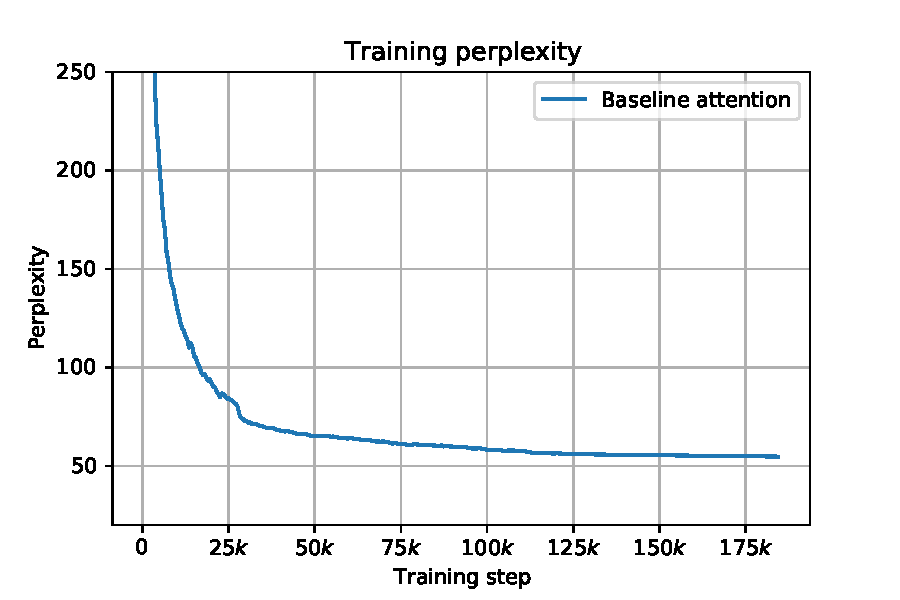
\includegraphics[height=8cm]{obrazky/train_baseline.pdf}
    \caption{Training perplexity progress of baseline solution}
    \label{fig:trainning_progress_baseline}
\end{figure}

\subsection{Performer model experiments}

Next we have chosen in order to compare results of classical attention and the FAVOR+ attention to train two net-works with equal hyper-parameters, only difference being in used attention mechanism. The network hyper-parameters are shown in the Table \ref{tab:paramshared}. The smaller network size is mainly due to performance requirements of performer network on smaller input sequence sizes.  In this smaller setting we have achieved only 129.4 perplexity for GPT variant and 129.2 perplexity for Performer variant, after 5 epochs of training, and can be seen on figure \ref{fig:trainningprogress}. Overall real time of training for GPT variant was 4 hours and 59 minutes, and for Performer it was 21 hours and 11 minutes. Next are examples of input sequences of:
\newpage
\subsubsection*{Performer}
\begin{verbatim}
INPUT:  In 1691 Moscow established
\end{verbatim}
\begin{verbatim}
OUTPUT: In 1691 Moscow established a in =ed was cont f gener 1950
        gener 1950 a in gener 1950ches gener F a in gener 1950 a 
        gener 1950ed was gener 1950 cont gener 1950 f gener 1950 
        a in gener 1950chchyl gener F a in gener 1950 F
\end{verbatim}

\subsubsection*{Transformer (Equivalent to performer parameters)}
\begin{verbatim}
INPUT:  In 1691 Moscow established
\end{verbatim}
\begin{verbatim}
OUTPUT: In 1691 Moscow established ecn = a =ivingently life =ed 
        Cionionionionionionionionion C was contol However
        Howeverionionionionionionion C was contol Howeverol 
        Howeverol However distributed contol However f 
        Republicecnired return f Republicecn =ch Republic
\end{verbatim}

\begin{table}[H]
    \centering
    \begin{tabular}{|c|c|c|c|c|c|}
    \hline
    Hyper-parameters & \texttt{vocab\_size} &  \texttt{d\_model} & \texttt{n\_layers} & \texttt{n\_heads} & \texttt{d\_ff} \\ \hline
    Values & 30 000 & 128 & 2 & 4 & 512\\ \hline
    \end{tabular}
    \caption{Shared architecture parameters for trained models.}
    \label{tab:paramshared}
\end{table}

\begin{figure}[H]
    \centering
    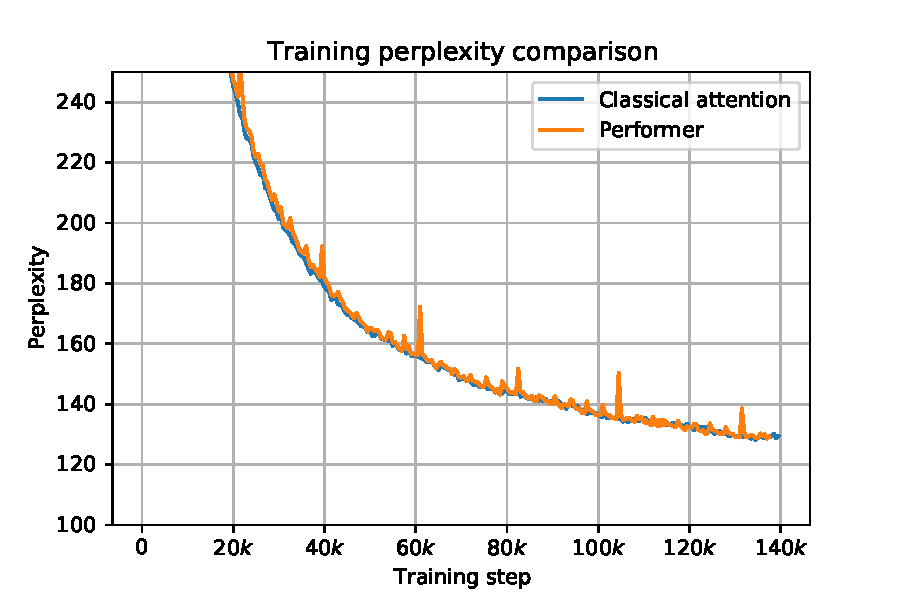
\includegraphics[height=8cm]{obrazky/train.pdf}
    \caption{Training perplexity progress with multi-head attention and performer}
    \label{fig:trainningprogress}
\end{figure}

%\begin{figure}[H]
%    \centering
%    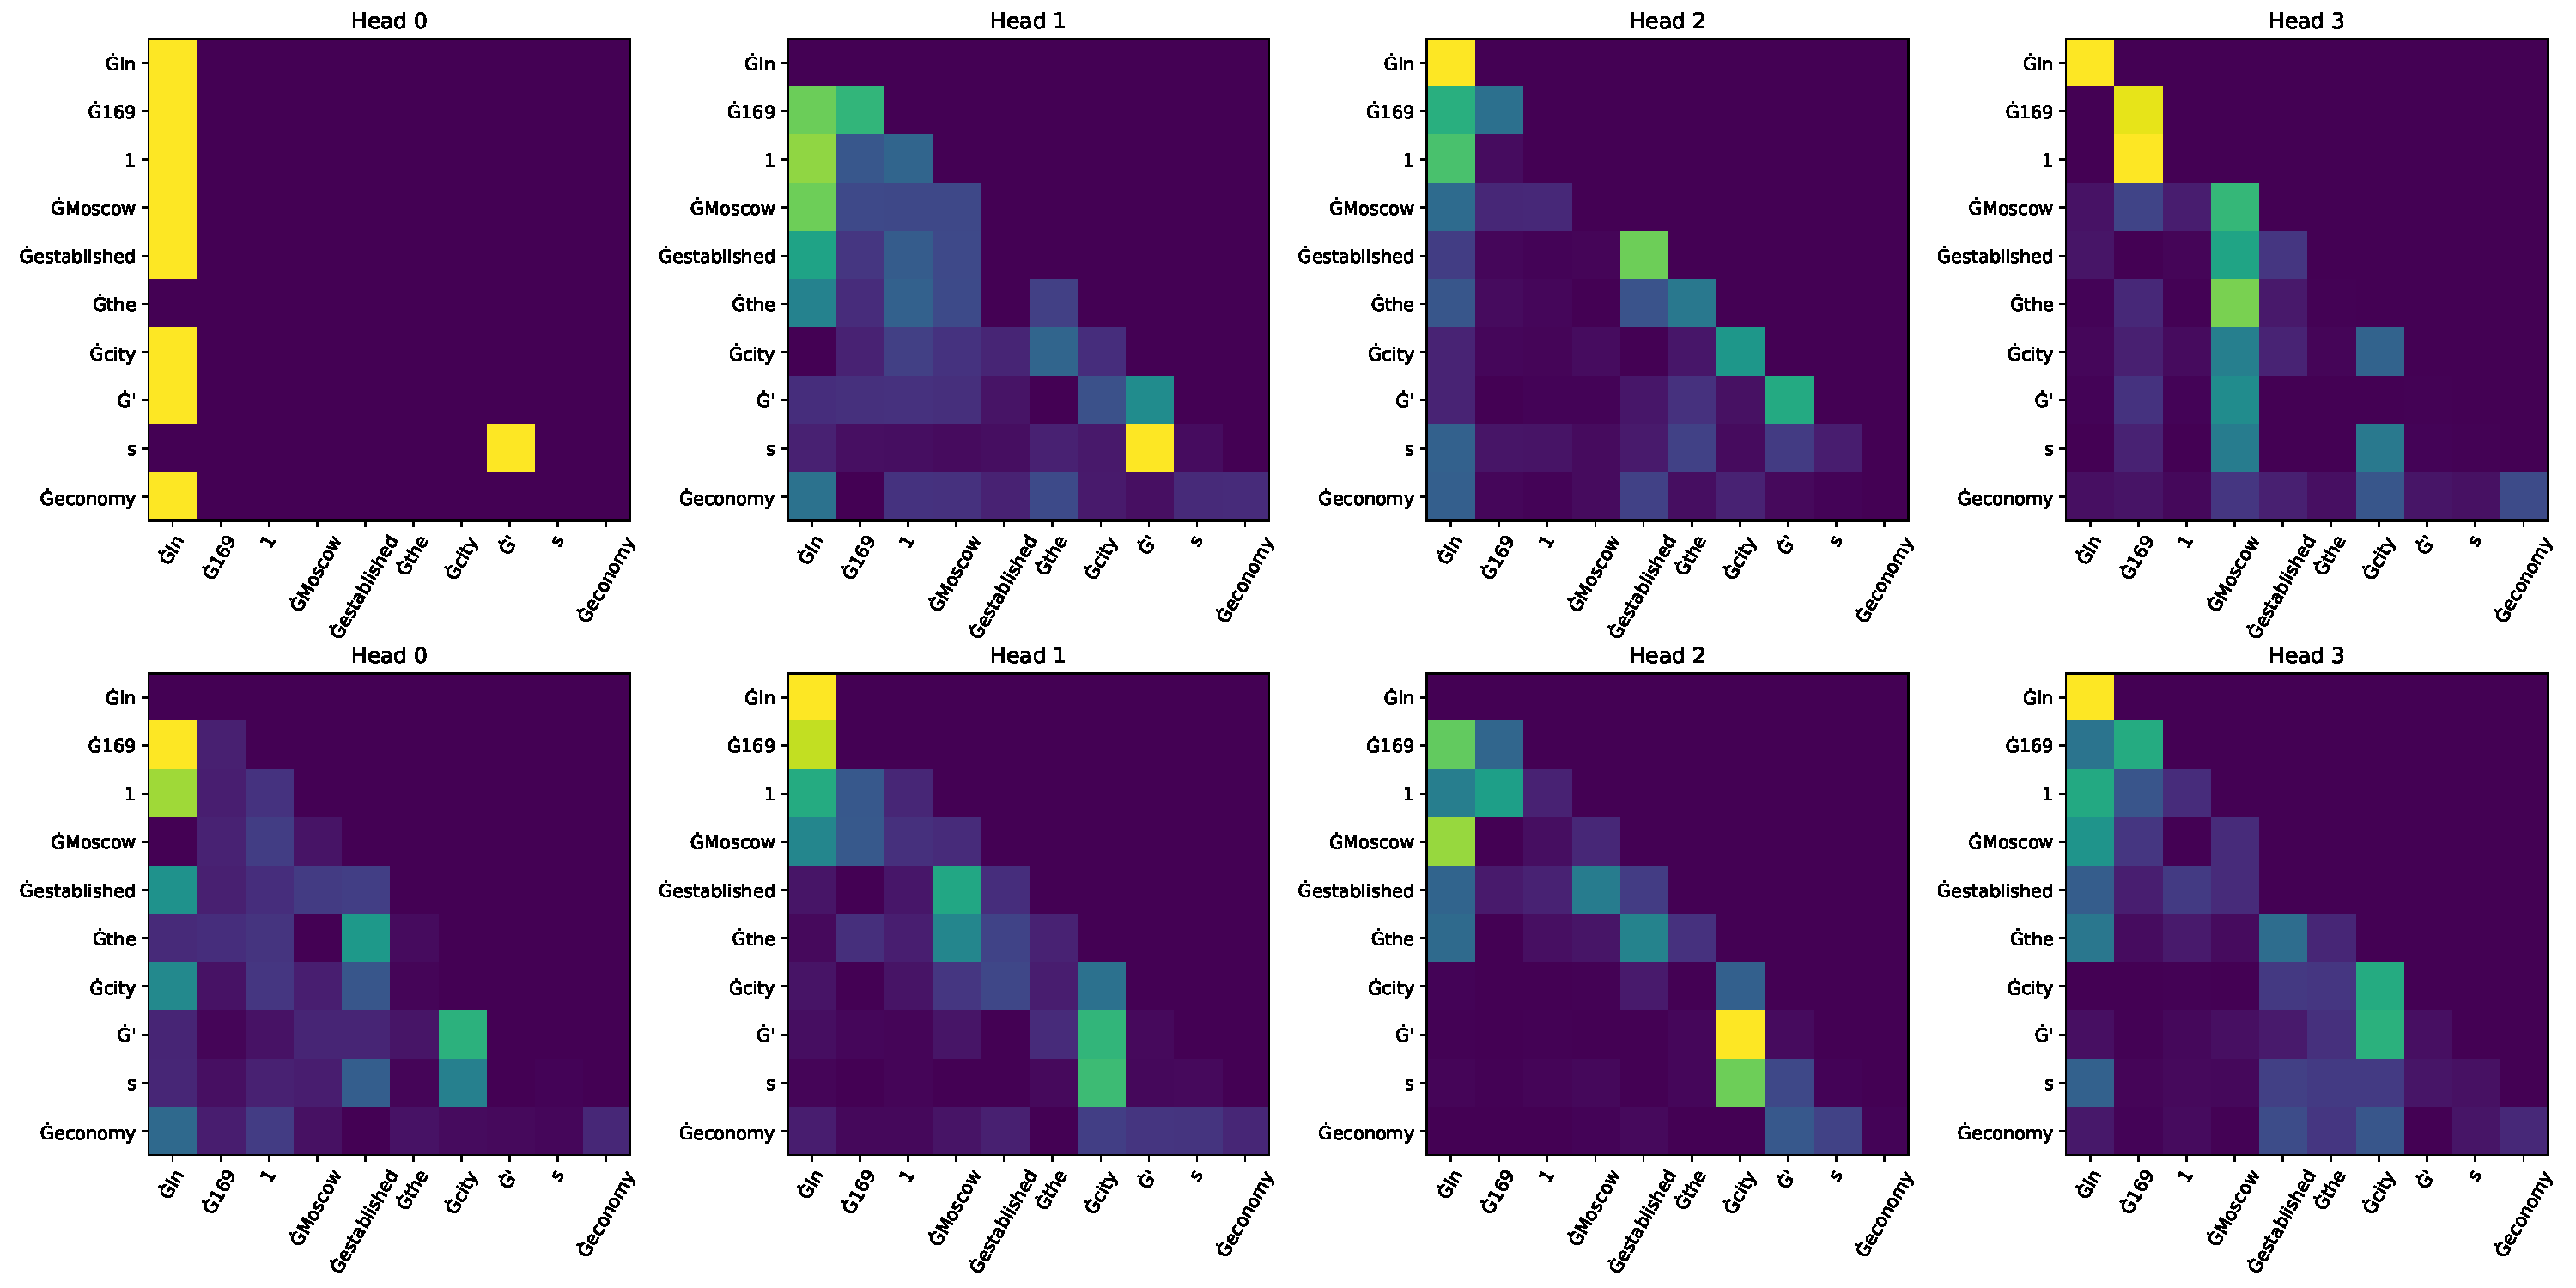
\includegraphics[width=16cm]{obrazky/AttentionWeights.pdf}
%    \caption{Attention weights for classical multi-head attention (by row layer 0, layer 1)}
%    \label{fig:my_label}
%\end{figure}
\newpage
\section{Conclusion}
Our work focused on creating language model using two different approaches. We have successfully implemented both attention and performer based language models and showed their train-ability. The attention model has shown upon experimentation promising results and has is able to generate coherent English sentences. Our experimentation using \textit{FAVOR+} algorithm has shown some of its limitations. Approach promises linear time and space complexity of attention approximation however it does not provide these advantages when smaller sequences are used. Thus our experimentation only allowed small models. These results are coherent with theoretical evaluation  where it is determined that time and space complexity with relation to sequence length is linear but it is quadratic with relation to embedding size. This is exactly opposite of classical attention. Our model used significantly larger embedding size an thus it could not benefit from advantages provided by \textit{FAVOR+}, which in return worsened its performance. 

The experimentation shows that wen equivalent performer and attention model size was used the results were similar. This can be seen in training progress graph but also with the similar output. The output has not been as good as with larger model size but if enough computational resources we would expect similar results. This can be said as training progress of both models is more less equivalent. 

Future experimentation may take advantage of larger memory size or by experimenting with different sizes of embedding. The linear time and space complexity can thus provide its advantages and allow training and evaluation on larger samples of data. 
